\documentclass[11pt]{report}
\usepackage[utf8]{inputenc}
\usepackage{geometry}
\usepackage{enumitem}
\usepackage{hyperref}
\usepackage{titlesec}
\usepackage{longtable}
\usepackage{multirow}
\usepackage{array}
\usepackage{amsmath}
\usepackage{titlepic}
\usepackage{titlesec}
\usepackage{graphicx}
\usepackage{xcolor}
\usepackage{float}
\usepackage{caption}
\usepackage{subcaption}
\usepackage{listings}

\hypersetup{
    colorlinks=true,
    linkcolor=black,
    filecolor=magenta,      
    urlcolor=blue,
}


\setlist[enumerate]{label*=.\arabic*}
\titleformat{\chapter}[display]
{\normalfont\bfseries}{}{0pt}{\Huge}
\geometry{a4paper, layoutwidth=24cm, layoutheight=32cm}
\addtolength{\hoffset}{-1.5cm}
\renewcommand*\contentsname{Indice}
\titlespacing{\chapter}{-0.2cm}{1.0cm}{1.0cm}
\title{Systems, Modelica, MPGOS and modelica2GPU}
\date{Ottobre, 2020}
\makeatletter
\let\documentTitle\@title
\let\academicYear\@date
\makeatother

\begin{document}
\begin{titlepage}
    \centering
    \textsc{\Large Università di Roma La Sapienza\\[.3cm]Facoltà di Ingegneria dell'informazione, informatica e statistica\\[.3cm]Dipartimento di Informatica}
    \vspace*{1cm}
    \hrule\hrule\hrule\hrule\hrule
    \vspace*{0.1cm}
    \hrule\hrule\hrule\hrule\hrule
    \vspace*{1cm}
    \textsc{\Huge L'uso della GPU nel MBSE}
    \vspace*{1cm}
    \hrule\hrule
    \vspace*{1cm}
    \textbf{\Large \documentTitle}
    \vspace*{1cm}
    \hrule\hrule\hrule\hrule
    \vspace*{3cm}
    \textsc{\large Riccardo La Marca 1795030}\\
    \vspace*{.2cm}
    {\large riccardo.lamarca98@gmail.com}\\
    \vspace*{.2cm}
    {\large lamarca.1795030@studenti.uniroma1.it}\\
    \vspace*{8cm}
    {\normalsize \academicYear}
\end{titlepage}
\tableofcontents
%% listings-modelica.cfg
%% Copyright 2014 Martin Sjoelund, Dietmar Winkler
%
% This work may be distributed and/or modified under the
% conditions of the LaTeX Project Public License, either version 1.3
% of this license or (at your option) any later version.
% The latest version of this license is in
%   http://www.latex-project.org/lppl.txt
% and version 1.3 or later is part of all distributions of LaTeX
% version 2005/12/01 or later.
%
% This work has the LPPL maintenance status `maintained'.
%
% The Current Maintainer of this work is Dietmar Winkler
%
% Code repository https://github.com/modelica-tools/listings-modelica
%
% This work consists of the file listings-modelica.cfg

\lstdefinelanguage{modelica}
{
  morekeywords=[1]{
    algorithm,and,annotation,as,assert,block,break,case,class,connect,connector,
    constant,constrainedby,der,discrete,each,else,elseif,elsewhen,encapsulated,
    end,enumeration,equality,equation,expandable,extends,external,failure,final,
    flow,for,function,guard,if,import,in,initial,inner,input,List,local,loop,
    match,matchcontinue,model,not,operator,Option,or,outer,output,package,parameter,
    partial,protected,public,record,redeclare,replaceable,return,stream,
    subtypeof,then,Tuple,type,uniontype,when,while},
  morekeywords=[2]{true, false},
  % Do not make true,false keywords because fn(true,x, false ) shows up as fn(true,x, *false*)
  morekeywords=[3]{optimization,constraint}, % Optimica keywords
  morekeywords=[4]{objective,startTime,finalTime,initialGuess},
  sensitive=true,
  comment=[l]//,
  morecomment=[s]{/*}{*/},
  alsodigit={.,-},
  morestring=[b]',
  morestring=[b]",
}[keywords,comments,strings]

\definecolor{keywordcolor1}{rgb}{0,0,.4}
\definecolor{keywordcolor2}{rgb}{.90,0,0}
\definecolor{keywordcolor3}{rgb}{.4,0,.8}
\definecolor{keywordcolor4}{rgb}{0.5,0,0.5}
\definecolor{stringcolor}{rgb}{0.133,0.545,0.133}
% \definecolor{listingbgcolor}{rgb}{0.95,0.95,0.95}

\lstset{
  breaklines=true,
  language=modelica,
  basicstyle=\ttfamily,
  keywordstyle=[1]\color{keywordcolor1}\bfseries,
  keywordstyle=[2]\color{keywordcolor2},
  keywordstyle=[3]\color{keywordcolor3}\bfseries,
  keywordstyle=[4]\color{keywordcolor4},
  stringstyle=\color{stringcolor},
%  backgroundcolor=\color{listingbgcolor},
  framexleftmargin=5pt,
  xleftmargin=5pt,
  xrightmargin=5pt,
  showstringspaces=false
}

\newcommand{\code}[1]{\lstinline|#1|}
\newcommand{\modelica}[1]{\lstinline[language=modelica]|#1|}

\newpage
\section*{Cos'è MBSE?}
\textbf{MBSE}, o Model-based System Engeenering, è una pratica dell'ingegneria dei sistemi secondo la quale la comunicazione tra i membri del team non avviene tramite documenti cartacei ma ben tramite lo sviluppo di modelli, solitamente tramite il linguaggio \textit{SysML} o \textit{UML}, per evitare abigiutà ed errori di interpretazione a causa del linguaggio naturale utilizzato. 
\chapter{Introduzione}
Sempre più, nella nostra realtà, sta diventando importante modellare e simulare \textit{sistemi cyber-fisici}, come droni o sistemi IoT, e \textit{sistemi biologici}, come il ciclo cellulare o ancora lo sviluppo e la propagazione di un virus. Sebbene questi due siano argomenti diversi, hanno principalmente una cosa in comune: entrambi possono essere espressi come un sistemi di equazioni differenziali (o \textit{ODE}, \textit{Ordinary Differential Equation}) il quale può essere integrato sul tempo al fine di dare un "vita" al modello stesso il quale risulterà in un dataset con cui si andrà a descrivere l'andamento, in termini di valori sugli stati, quindi la \textbf{traiettoria} del sistema stesso. Questa fase di integrazione viene chiamata \textit{simulazione} del modello, durante la quale vengono ad essere scoperti i valori sugli stati, calcolati a seguito del processo di integrazione delle derivate e di valutazione di particolari situazioni che vengono dette \textbf{eventi}.

Gli \textit{eventi} sono delle situazioni alternative che deviano il normale corso della traiettoria del sistema facendole toccare punti che altrimenti non avrebbero mai considerato. Esistono quindi due tipologie di eventi: di \textit{stato} e di \textit{tempo}. I primi sorgono da condizioni sugli stati, ad esempio $x > 10$ con $x$ stato del sistema, mentre i secondi da condizioni sul tempo. Su quest'ultimi il discorso diventa più ampio però un classico evento di questo tipo scaturisce inserendo nel sistema una componente detta \textit{Sample-And-Hold}, che agisce creando una condizione sul tempo della simulazione. Una componente di \textit{Sample-And-Hold}, letteralmente "campionamento e mantenimento" è una classica componente che viene inserita all'intero di sistemi continui al fine di discretizzarne una parte di comportamento. Il nome stesso deriva dalle due azioni che questo svolge: (1) campiona il tempo della simulazione in base a dei valori che per semplicità chiameremo $start$ ed $interval$, e (2) mantiene fino al prossimo sample il valore di uno stato. Un tipico esempio è l'\textbf{Analog to Digital Converter} (ADC) il quale implementa internamente il sottosistema di s\&h\footnote{Sample-And-Hold}. Gli eventi, quindi, servono principalmente per immettere una discretizzazione all'interno di un sistema che altrimenti sarebbe continuo.\\

\begin{figure}[h]
    \centering
    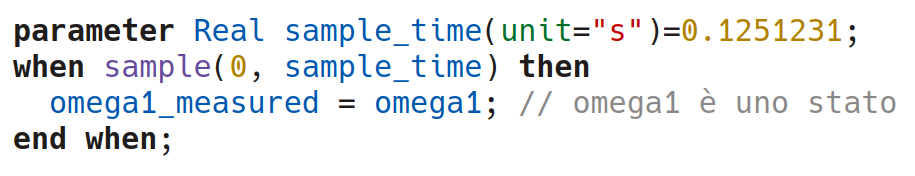
\includegraphics[width=120mm]{Intro/SH.png}
    \caption{Esempio di componente SH in Modelica.}
    \label{fig:SampleAndHoldComponentModelica}
\end{figure}
\newpage
\subsection*{Esempio1. First order system with sample-and-hold}
Si consideri il semplice sistema descritto da una sola equazione differenziale\footnote{Scriveremo $\dot{x}$ al posto di $\frac{\mathrm{d}}{\mathrm{d}t}x(t)$}.
\begin{equation}
    \dot{x} = (1 - x)
\end{equation}
Vediamo come questo sistema descrive semplicemente l'andamento dello stato x fino al punto 1, sul quale troverà l'equilibrio dal momento che per tutti i successivi istanti di tempo non cambierà mai di valore. Difatti il grafico della traiettoria sarà il seguente\\
\begin{figure}[h]
    \centering
    \begin{subfigure}[b]{0.4\textwidth}
        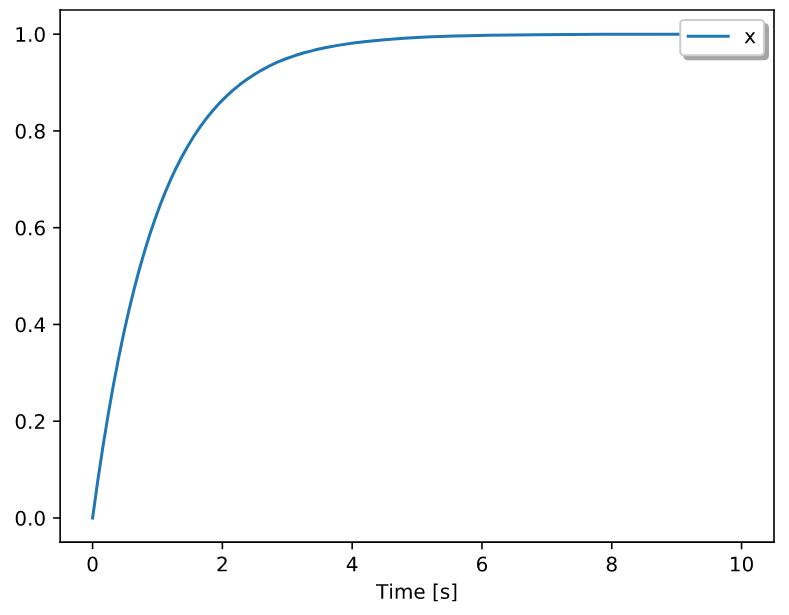
\includegraphics[width=\textwidth]{Intro/FirstOrderSystem_a.png}
        \caption{Traiettoria del sistema con valore iniziale $x=0$}
        \label{fig:my_label}
    \end{subfigure}
    \begin{subfigure}[b]{0.4\textwidth}
        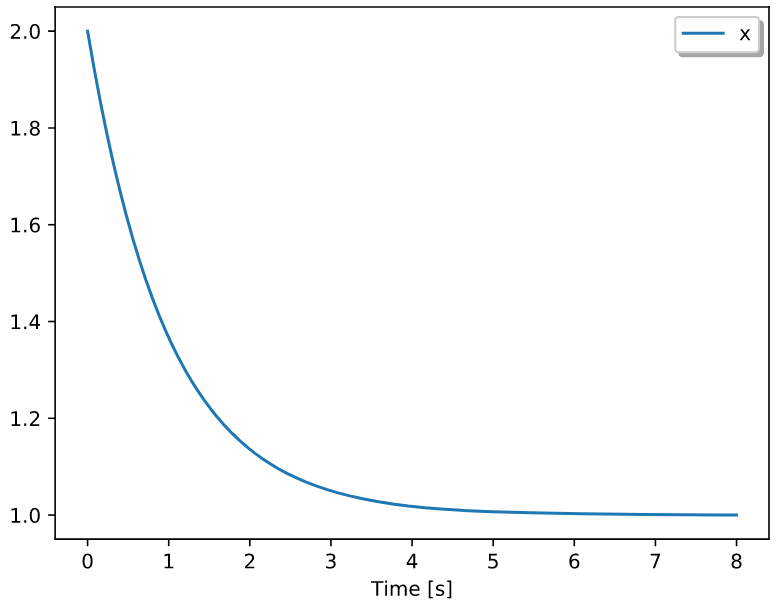
\includegraphics[width=\textwidth]{Intro/FirstOrderSystem_b.png}
        \caption{Traiettoria del sistema con valore iniziale $x=2$}
        \label{fig:my_label}
    \end{subfigure}
\end{figure}
Se volessimo aggiungere una componente SH all'interno del sistema per vedere il valore di $x$ a determinati istanti di tempo, decidiamo prima il tempo di sampling (es. 0.3) e implementiamo tale evento, ottenendo

\begin{figure}[!h]
    \centering
    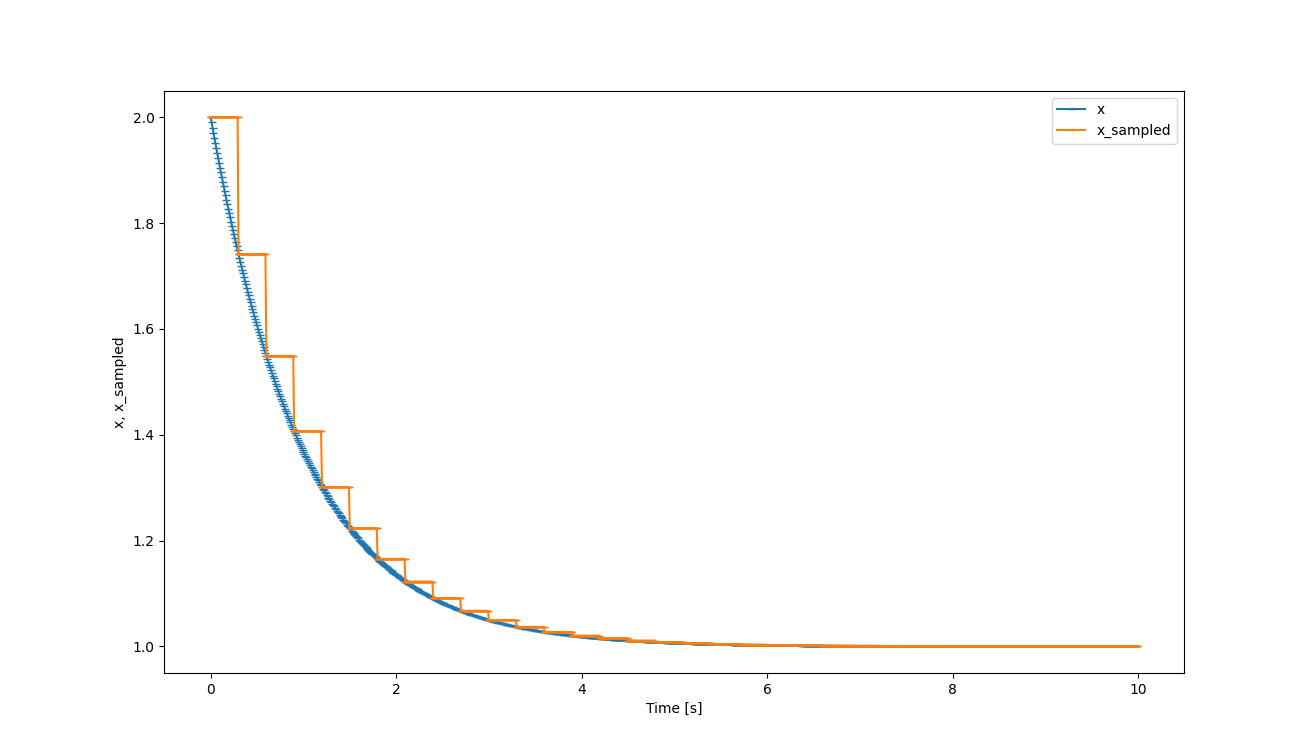
\includegraphics[width=\textwidth, height=70mm]{Intro/Plot.png}
    \caption{FirstOrderSystem con sample-and-hold e sample time di 0.3}
    \label{fig:my_label}
\end{figure}
%\subsection*{Esempio2. Second order system with sample-and-hold}
%Iniziamo considerando un 

\end{document}
